
\documentclass[12pt]{article}

\usepackage[margin=1in]{geometry}
\usepackage[T1]{fontenc}
\usepackage[utf8]{inputenc}
\usepackage{mathptmx}
\usepackage{setspace}
\usepackage{titlesec}
\usepackage{tocloft}
\usepackage{array}
\usepackage{longtable}
\usepackage{booktabs}
\usepackage{enumitem}
\usepackage{caption}
\usepackage{graphicx}
\usepackage{float}
\usepackage[hidelinks]{hyperref}
\usepackage{multirow}
\usepackage{xurl}
\usepackage{fancyhdr}
\usepackage{titling}
\usepackage[T1]{fontenc}
\usepackage{lmodern}
\setstretch{1.08}
\setlength{\parskip}{0.35em}
\setlength{\parindent}{0pt}

\titleformat{\section}{\large\bfseries}{\thesection}{0.75em}{}
\titleformat{\subsection}{\normalsize\bfseries}{\thesubsection}{0.75em}{}
\titleformat{\subsubsection}{\normalsize\bfseries}{\thesubsubsection}{0.75em}{}

\pagestyle{fancy}
\fancyhf{}
\fancyfoot[C]{\thepage}
\renewcommand{\headrulewidth}{0pt}

\begin{document}

\begin{titlepage}
\centering
\vspace*{0.3cm}

\includegraphics[width=0.38\textwidth]{figs/gw_logo.png}\par

\vspace{1.2cm}

{\large Data Science Program\par}
\vspace{0.6cm}

{\large Capstone Report - Spring 2026\par}
\vspace{1.6cm}

{\LARGE \textbf{BRIDGE: Building Role-Specific Interprofessional Dialogue and Guided Education}\par}
\vspace{1.4cm}

{\large Hari Prasannaa Thangavel Ravi,\\
Anusha Umashankar\par}
\vspace{1cm}

{supervised by\\
Prof. Amir Jafari and Prof. Andrew Wiss}
\vspace{1cm}

{\normalsize Date: April 2026\par}

\vfill

% {\large \textbf{Abstract}\par}

\newpage
\begin{center}
\Large\textbf{Abstract}
\end{center}
\vspace{0.5cm}

\begin{minipage}{0.88\textwidth}
\small
BRIDGE is an AI-powered, multi-agent conversational system designed to simulate interprofessional collaboration in healthcare education. The system consists of six professional agents, each representing a healthcare role and responding to clinical scenarios from its own perspective using a large language model (LLM). To improve reliability and reduce hallucinations, BRIDGE integrates a Retrieval-Augmented Generation (RAG) pipeline that grounds responses in verified opioid-domain clinical literature instead of relying solely on the LLM's parametric knowledge. This report evaluates two key design decisions that significantly impact RAG performance: how source documents are split into retrievable chunks and which embedding model is used to match student queries to relevant chunks. Multiple chunking strategies were evaluated, including fixed chunking, fixed chunking with overlap, recursive chunking, semantic chunking, and sentence-based chunking. These experiments showed that a chunk size of 7000 tokens and retrieval depth of $k = 7$ performed especially well, offering a strong balance between retrieval quality, contextual coverage, and efficiency. These parameters were therefore selected for the BRIDGE RAG pipeline. Seven retrieval models, including both dense and sparse approaches, were benchmarked at $k = 7$ under different retrieval modes. Results indicate that BGE-M3 achieves the strongest dense retrieval performance, while BM25 provides a highly competitive and efficient baseline. In addition, metadata-based profession filtering emerged as an important architectural component for maintaining role-specific retrieval quality and ensuring that each agent accesses evidence relevant to its scope of practice.
\end{minipage}
\end{titlepage}

\tableofcontents
\newpage

\section{Introduction}

Interprofessional collaboration is essential in healthcare, but students often do not receive enough exposure to how different professions work together in real clinical scenarios. In many cases, education is still siloed, with each discipline learning separately rather than learning how to communicate, coordinate, and make decisions as a team.

BRIDGE addresses this gap by simulating a team of healthcare professionals using AI agents. Each agent represents a specific role and provides responses aligned with its expertise, allowing students to compare how different professionals would approach the same case. The system particularly emphasizes opioid-related scenarios, where precise, evidence-based, and role-specific decision-making is crucial.

The main objective of this project is to strengthen BRIDGE through the integration of a Retrieval-Augmented Generation (RAG) pipeline. By retrieving relevant clinical evidence and grounding responses in external sources, BRIDGE becomes more accurate, more current, and more educationally useful.

The report focuses on the design and evaluation of the retrieval layer that enables BRIDGE to support clinically grounded, role-specific responses. In particular, the project studies how chunking strategy, retrieval depth, embedding-model choice, and metadata filtering affect the quality of evidence supplied to each professional agent.

\section{Problem Statement}

Healthcare students need opportunities to observe how different professionals reason about the same clinical case, yet live interprofessional exercises are difficult to scale because they require coordination across programs, instructors, and schedules. A digital alternative must therefore do more than simply generate fluent answers: it must preserve role distinctions, remain aligned with current clinical guidance, and reduce the risk of hallucinated claims in a safety-sensitive domain.

The specific problem addressed in this project is how to build a retrieval-augmented, multi-agent educational system that can surface profession-specific evidence reliably enough to support opioid-focused case discussions. This requires solving several challenges simultaneously: curating a clinically meaningful evidence base, converting heterogeneous PDF and web content into retrievable text, selecting chunking strategies that balance context against precision, choosing retrieval models that perform well on a small specialized corpus, and designing metadata filters that maintain role-specificity without unnecessarily excluding relevant evidence.

\section{Related Work}

\subsection{Retrieval-Augmented Generation}

RAG was introduced to combine the parametric memory of a pre-trained language model with a non-parametric external store, allowing the model to cite current evidence rather than reproduce what it memorized during training \cite{lewis2020rag}. Izacard and Grave extended the idea with Fusion-in-Decoder, which encodes multiple retrieved passages independently before decoding \cite{izacard2021fid}. The survey by Gao et al. catalogues the maturation of the area into naive, advanced, and modular variants, with most recent research focused on improving retrieval precision, handling multi-hop queries, and reducing prompt-length overhead \cite{gao2023ragsurvey}.

Chunking strategy receives less formal attention in the literature than it deserves. Practitioner-oriented work has converged on a small set of heuristics --- fixed-size windows, recursive character splitters, and embedding-based semantic splitting --- that are widely implemented in frameworks such as LangChain and LlamaIndex \cite{langchain2023,kamradt2023}. More recent academic work on late chunking and small-to-big retrieval demonstrates that the boundary between chunking and retrieval is itself a research object \cite{gunther2024late}. Our evaluation takes a pragmatic view: rather than propose a new chunker, we measure how five established strategies behave across a clinical corpus.

\subsection{Embedding Models for Dense Retrieval}

Dense retrievers rank passages using the cosine similarity of learned vector representations. Sentence-BERT \cite{reimers2019sbert} and MPNet \cite{song2020mpnet} established the practical viability of transformer-based sentence encoders. More recent models such as the BGE family \cite{xiao2023bge,chen2024bgem3} and E5 \cite{wang2022e5} have improved retrieval accuracy on general-domain benchmarks. Sparse lexical methods remain competitive. BM25 in particular continues to set a strong baseline on tasks where exact term overlap matters \cite{robertson2009bm25}, and recent studies caution against assuming dense retrievers dominate without case-specific evidence \cite{thakur2021beir}. Our comparison includes both families to avoid that assumption.

\subsection{Multi-Agent LLM Systems}

Orchestrating several LLM-backed agents to play distinct roles is an active research area. Generative agents were shown to produce plausible human-like behaviour in simulated social settings \cite{park2023generative}. Frameworks such as AutoGen \cite{wu2023autogen} and CAMEL \cite{li2023camel} formalize multi-agent conversation for programming and problem-solving tasks. The IPE context differs in an important way: the goal is not to reach consensus efficiently, but to surface role-specific reasoning so that a human student can compare perspectives. We therefore design BRIDGE to run agents in parallel rather than have them negotiate.

\subsection{AI for Healthcare Education}

LLMs fine-tuned or prompted for medical tasks --- MedPaLM \cite{singhal2023medpalm}, BioBERT \cite{lee2020biobert}, and others --- have demonstrated strong performance on medical question-answering benchmarks. Evidence from the education literature is thinner. Studies of virtual standardized patients date back to the pre-LLM era \cite{stevens2006virtual}, and recent work has begun to examine LLM-based tutors in specific clinical domains. To our knowledge, a per-agent, profession-partitioned RAG architecture for IPE has not been reported, and the trade-offs explored here have not been quantified on an opioid-education corpus.



\section{System Overview}

BRIDGE is a multi-agent conversational system where each agent is powered by an LLM and produces role-specific responses to clinical queries. The system is designed to simulate realistic interprofessional discussion by showing students how different healthcare roles interpret and respond to the same patient scenario.

The system integrates Retrieval-Augmented Generation (RAG) so that responses are grounded in clinical evidence rather than being generated only from pretrained model knowledge.

\subsection{Existing System Architecture}

The BRIDGE baseline system is built as a web-based multi-agent platform with the following components:

\begin{itemize}[leftmargin=1.5em]
    \item Backend: FastAPI (Python)
    \item LLM: GPT-4o
    \item Database: PostgreSQL
    \item Execution model: Asynchronous parallel agent execution
\end{itemize}

Each selected agent processes the same query independently, allowing simultaneous generation of multiple profession-specific perspectives. This design supports side-by-side comparison of professional reasoning and improves the educational value of the platform.

\begin{figure}[H]
\centering
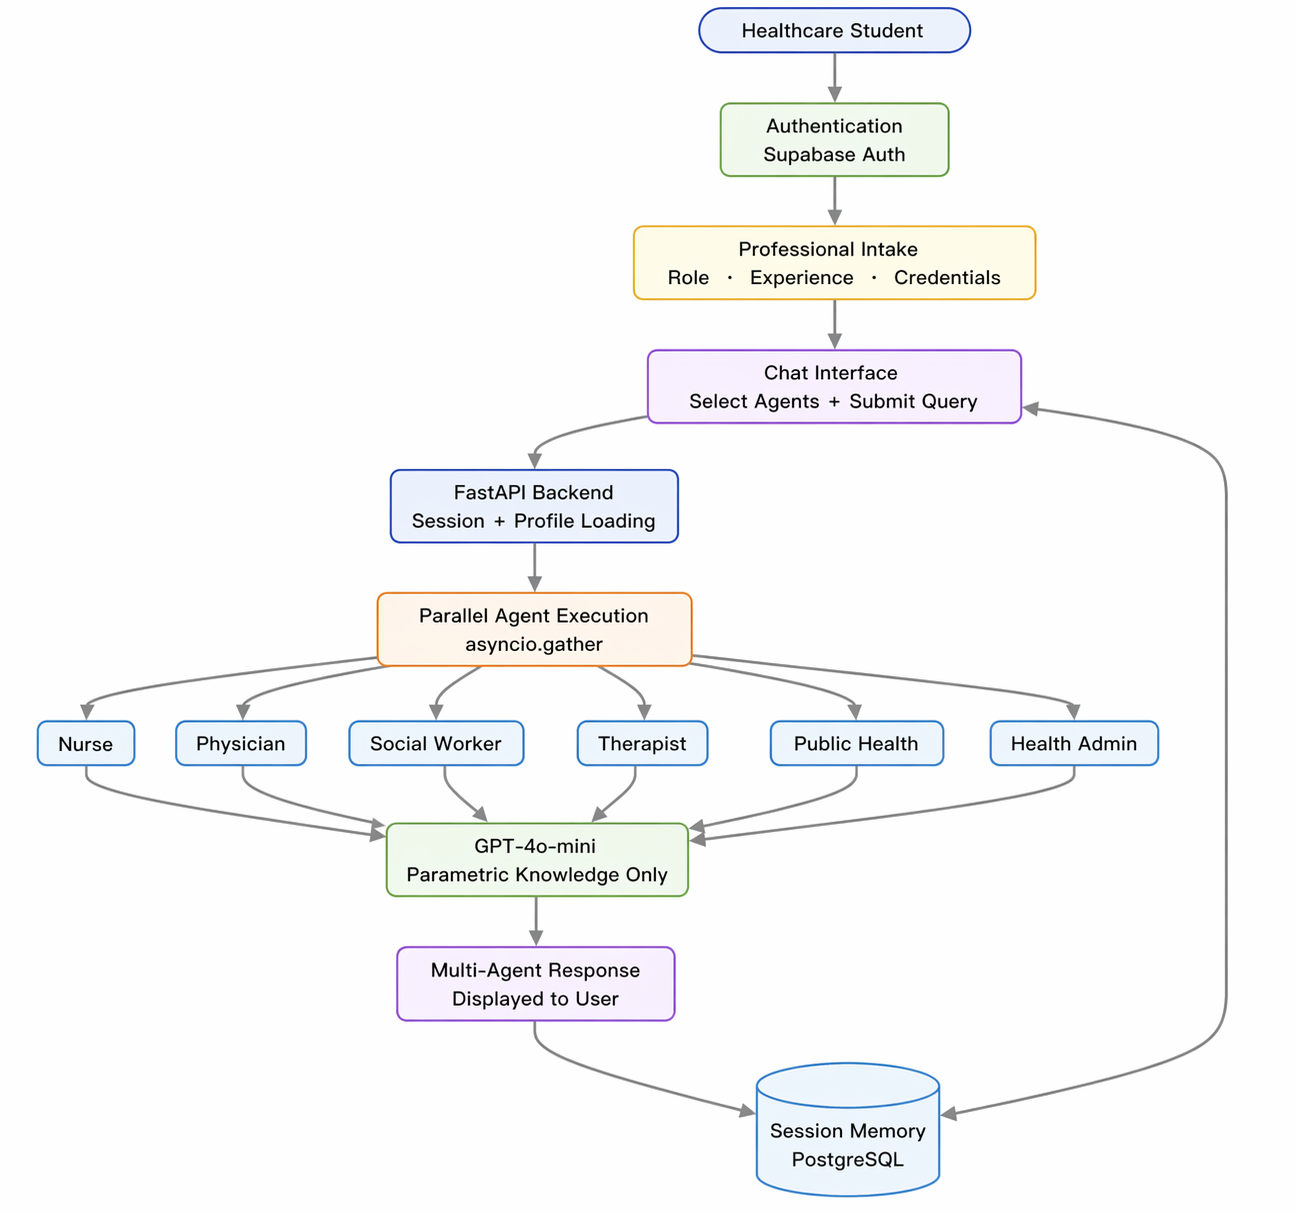
\includegraphics[width=0.72\textwidth]{figs/current_architecture.png}
\caption{Baseline BRIDGE system architecture. The figure illustrates how an authenticated student query is passed through the backend and dispatched to selected role-specific agents in parallel.}
\label{fig:baseline_architecture}
\end{figure}

The baseline architecture shown in Figure~\ref{fig:baseline_architecture} highlights an important limitation of the original system: each agent depends primarily on parametric model knowledge. This motivates the retrieval-grounded extensions described later in the report.

\subsection{Limitations of the Baseline System}

Although the baseline system is useful, it has several limitations:

\begin{itemize}[leftmargin=1.5em]
    \item No grounding in external knowledge
    \item Risk of hallucinated clinical facts
    \item Dependence on static prompts
    \item Limited ability to adapt to changing guidelines
    \item No retrieval evaluation framework
    \item Limited scenario scope
\end{itemize}

These limitations motivated the integration of an RAG pipeline and a more systematic retrieval evaluation.

\subsection{Professional Agents}

Each BRIDGE agent is defined by a carefully designed system prompt that encodes its professional identity, scope of practice, and communication style. The agents are not simple copies of the same model with different titles. Instead, each one is shaped to reflect a distinct clinical perspective.

This ensures meaningful variation across responses. For example, the nurse focuses more on patient observation, safety, and bedside care, while the physician assistant focuses on diagnosis and treatment planning. Similarly, the medical social worker emphasizes community resources and social determinants of health.

\begin{center}
\begin{tabular}{>{\raggedright\arraybackslash}p{2.2in} >{\raggedright\arraybackslash}p{3.2in}}
\toprule
\textbf{Agent} & \textbf{Clinical Focus} \\
\midrule
Nurse & Patient care, safety, bedside observations \\
Physician Assistant & Diagnostics, treatment planning \\
Medical Social Worker & Social care, community resources \\
Physical Therapist & Rehabilitation and recovery \\
Public Health Professional & Prevention, population health \\
Health Administrator & Policy, coordination \\
\bottomrule
\end{tabular}
\end{center}

These six roles collectively cover the continuum of care in opioid-related cases, from acute overdose management to long-term rehabilitation, prevention, and system-level response.

\subsection{Role of RAG}

Without RAG, each response depends entirely on the model's internal knowledge. This approach is not sufficient in a clinical setting because:

\begin{itemize}[leftmargin=1.5em]
    \item Medical guidelines change frequently
    \item Regulations vary by region and organization
    \item LLMs can confidently produce incorrect information
\end{itemize}

In opioid-related education, such errors can be harmful because they may lead students to absorb inaccurate clinical reasoning.

RAG addresses this problem by retrieving relevant evidence from a curated opioid-domain corpus and injecting it into the prompt. In this design, the LLM is no longer the sole source of factual information. Instead, it becomes an evidence synthesizer that reasons over retrieved passages.

This provides three major benefits:

\begin{enumerate}[leftmargin=1.5em]
    \item Accuracy: Responses are grounded in trusted sources such as CDC, SAMHSA, FDA, NIDA, and related clinical literature.
    \item Per-agent specialization: Each profession retrieves evidence relevant to its own role, reinforcing realistic professional boundaries.
    \item Updatability: New evidence can be added to the corpus without retraining the model.
\end{enumerate}

\subsection{Proposed RAG Architecture}

The BRIDGE RAG pipeline follows a per-agent retrieval architecture. When a user submits a query, the system routes it to the selected agents in parallel. Each agent then performs its own retrieval process over the evidence corpus.

The retrieved chunks are not directly appended to a fixed static prompt. Instead, BRIDGE uses a two-stage prompt generation design:

\begin{enumerate}[leftmargin=1.5em]
    \item The retrieved chunks are first sent to an LLM to generate a dynamic prompt tailored to the retrieved evidence and the selected profession.
    \item That generated prompt is then sent again to the LLM, together with the user's query and content, to produce the final response.
\end{enumerate}

This design improves flexibility over a static prompt template because the intermediate prompt can adapt to the specific evidence retrieved for that case. It also helps organize large retrieved contexts before the final answer is generated.

\textbf{Pipeline}

\begin{enumerate}[leftmargin=1.5em]
    \item The student submits a query.
    \item The query is routed to selected agents in parallel
    \item Each agent performs profession-filtered retrieval
    \item Top-$k$ chunks are retrieved
    \item Retrieved chunks are passed to an LLM to generate a dynamic evidence-based prompt
    \item The generated prompt, along with user content, is passed again to the LLM
    \item The final profession-specific response is generated
\end{enumerate}

This architecture supports role-aware, evidence-grounded, and context-sensitive response generation.

\begin{figure}[H]
\centering
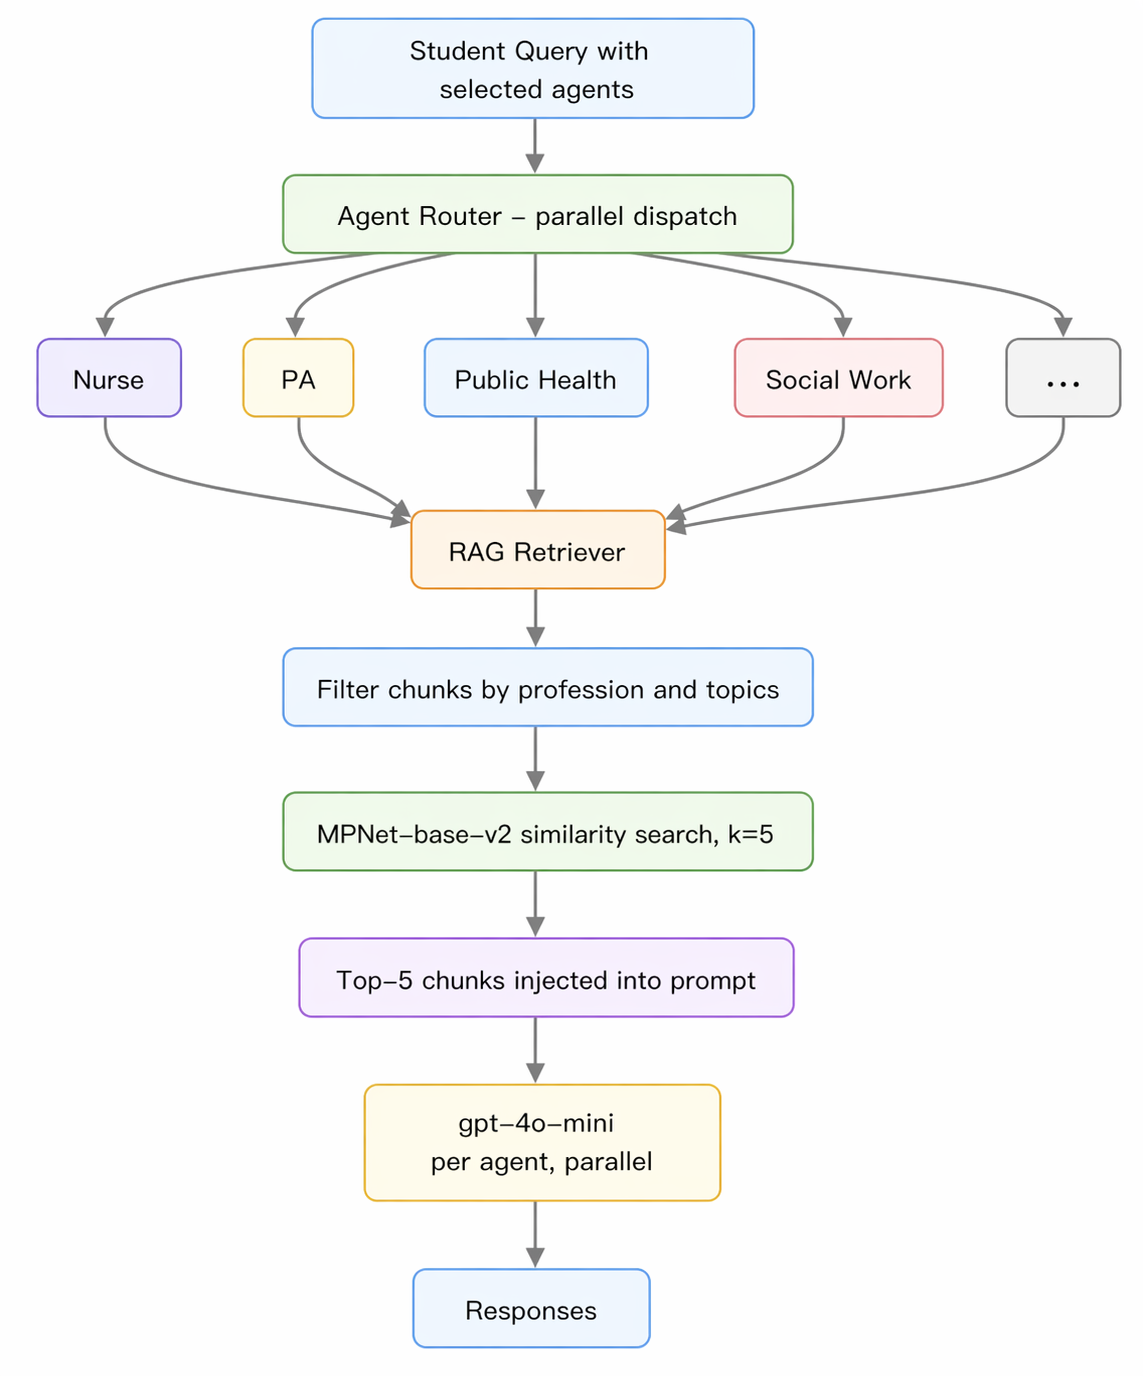
\includegraphics[width=0.62\textwidth]{figs/rag_flow.png}
\caption{Proposed per-agent RAG workflow. The query is routed to selected agents, filtered by metadata, matched against the evidence corpus, and used to construct evidence-grounded responses.}
\label{fig:rag_flow}
\end{figure}

Figure~\ref{fig:rag_flow} makes explicit that retrieval is embedded inside each agent's execution path rather than handled once globally. This per-agent design is important because it allows different healthcare roles to access different evidence slices and maintain realistic scope-specific reasoning.

\section{Data Pipeline}

\subsection{Data Sources}

The BRIDGE knowledge base was built from both PDF documents and web-based clinical resources focused on opioid-related care.

The corpus includes:

\begin{itemize}[leftmargin=1.5em]
    \item 45 PDF documents
    \item 30 web URLs
\end{itemize}

These sources were selected to provide broad coverage of clinical guidelines, treatment recommendations, public health resources, support services, and administrative perspectives relevant to opioid-related education.

\begin{center}
\begin{tabular}{>{\raggedright\arraybackslash}p{1.6in} c >{\raggedright\arraybackslash}p{3.0in}}
\toprule
\textbf{Source Type} & \textbf{Count} & \textbf{Description} \\
\midrule
PDFs & 45 & Clinical guidelines, research papers, reports, training materials \\
Web URLs & 30 & Public health pages, clinical references, guidance pages \\
Total Sources & 75 & Combined evidence corpus \\
\bottomrule
\end{tabular}
\end{center}

\textbf{Discussion}

The PDF sources contribute more detailed and structured long-form content, such as federal guidelines, formal publications, and technical reports. These are useful for capturing deep clinical knowledge and comprehensive treatment recommendations.

The web sources provide more accessible and updated content from public health organizations and clinical information portals. These are useful for covering practical guidance, patient education resources, and rapidly updated recommendations.

Together, the PDF and web sources create a balanced corpus that supports both depth and breadth of retrieval.

\subsection{Document Processing}

The source documents undergo several preprocessing steps before they are indexed:

\begin{itemize}[leftmargin=1.5em]
    \item Text extraction from PDFs
    \item Removal of repeated headers, footers, and formatting noise
    \item Normalization of spacing and line breaks
    \item Flattening of tables into plain text
    \item Cleaning and validation of extracted content
\end{itemize}

This preprocessing is necessary because PDF files are designed for visual presentation rather than structured retrieval. The extracted text is then prepared for chunking and embedding.

\subsection{Metadata Tagging}

Each chunk in the corpus is tagged with metadata to support targeted retrieval and analysis. Typical metadata fields include:

\begin{itemize}[leftmargin=1.5em]
    \item Profession label
    \item Topic category
    \item Source type
    \item Source title
    \item Chunk index
    \item Word or token count
    \item Source identifier
\end{itemize}

These metadata fields are especially important for profession-based filtering, which is a key part of the BRIDGE retrieval design.

\subsection{Profession Categorization}

Each source document is tagged with one or more profession labels so that the corpus can be filtered according to the selected agent. A single document may be relevant to multiple disciplines and is therefore allowed to carry multiple profession tags. This organization supports the instructional goal of BRIDGE by ensuring that retrieved evidence can remain aligned with professional scope of practice.

\begin{center}
\begin{tabular}{>{\raggedright\arraybackslash}p{2.3in} c}
\toprule
\textbf{Profession} & \textbf{Approximate Chunks} \\
\midrule
Public Health Professional & $\sim 48$ \\
Physician Assistant & $\sim 41$ \\
Nurse & $\sim 38$ \\
Medical Social Worker & $\sim 21$ \\
Physical Therapist & $\sim 6$ \\
Health Administrator & $\sim 5$ \\
General & $\sim 30$ \\
\bottomrule
\end{tabular}
\end{center}

The approximate distribution shows that public health, physician assistant, and nursing materials account for the largest share of the current corpus, while physical therapy and health administration remain smaller specialization areas. This imbalance reflects the present opioid-focused emphasis of the dataset and also points to future expansion opportunities.

\subsection{Opioid Topic Taxonomy}

In addition to profession labels, chunks are tagged with coarse opioid-domain topics. These tags support downstream analysis and help interpret retrieval behavior, although they are less reliable than manually curated profession labels for production filtering.

\begin{center}
\small
\begin{tabular}{>{\raggedright\arraybackslash}p{1.45in} >{\raggedright\arraybackslash}p{4.3in}}
\toprule
\textbf{Topic} & \textbf{Representative Keywords} \\
\midrule
Overdose & overdose, unresponsive, unconscious \\
Emergency & call 911, life-threatening, emergency \\
Naloxone & naloxone, narcan, intranasal \\
Withdrawal & withdrawal, detox, taper, physical dependence \\
Dosage & dosage, mg, milligram, titrate, twice daily \\
Treatment & buprenorphine, methadone, MOUD, OUD \\
Prevention & harm reduction, prevention, safe storage \\
Mental Health & mental health, depression, PTSD \\
Legal & controlled substance, schedule, HIPAA \\
Patient Education & patient education, caregiver, warning signs \\
\bottomrule
\end{tabular}
\end{center}

\subsection{Extraction Pipeline Details}

Most clinically relevant guidance documents are distributed as PDFs, which are designed for visual presentation rather than clean downstream retrieval. During development, multiple PDF extractors were considered. Faster tools such as PyPDF were useful for basic extraction but were less reliable on multi-column layouts and complex tables. Other tools improved certain edge cases, but the final extraction choice favored layout preservation and reading-order consistency.

Docling was adopted as the primary PDF extraction approach because it preserved tables, layout, and reading order more reliably for the current corpus. For web-based sources, the extraction process normalized fetched HTML into readable text segments before chunking. This preprocessing step is important because the quality of retrieval depends directly on the quality and coherence of the text that enters the chunking stage.

\subsection{Experimental Setup}

The chunking evaluation explored five chunking methods across four target token sizes (3000, 5000, 7000, and 10000) and four retrieval depths ($k \in \{3,5,7,9\}$), yielding 80 configurations in total. Embedding-model comparison was then performed at the selected retrieval depth of $k=7$ using a held-out set of representative student queries. For embedding comparison, Mean Reciprocal Rank (MRR), Precision@$k$, Recall@$k$, and F1@$k$ were treated as the primary metrics. MRR was especially important because the highest-ranked chunks are the most likely to influence downstream generation.

\section{Chunking Strategy}

\subsection{Approaches Evaluated}

Five chunking approaches were evaluated:

\begin{itemize}[leftmargin=1.5em]
    \item Fixed chunking
    \item Fixed chunking with overlap
    \item Recursive chunking
    \item Semantic chunking
    \item Sentence-based chunking
\end{itemize}

These methods were tested across different token sizes and retrieval depths to understand how chunk granularity affects retrieval quality.

\subsection{Evaluation Metrics}

The chunking strategies were compared using:

\begin{itemize}[leftmargin=1.5em]
    \item Hit Rate
    \item Average First Hit Rank
    \item Query latency
    \item Number of chunks generated
    \item Chunk build time
    \item Index build time
\end{itemize}

These metrics help evaluate both retrieval effectiveness and system efficiency.

\subsection{Chunking Results and Analysis}

Experiments indicated that retrieval quality depends strongly on the trade-off between chunk size and retrieval depth.

\begin{itemize}[leftmargin=1.5em]
    \item Smaller chunks provide more precise retrieval but may break context into pieces.
    \item Larger chunks preserve more context but can introduce irrelevant information into the retrieved results.
\end{itemize}

The chunking experiments indicated that 7000-token chunks consistently performed well because they preserved enough clinical context while keeping the number of chunks manageable. Likewise, $k = 7$ was found to be a strong retrieval depth because it provided high coverage without unnecessarily increasing prompt size.

\begin{center}
\begin{tabular}{>{\raggedright\arraybackslash}p{1.7in} >{\raggedright\arraybackslash}p{2.2in} >{\raggedright\arraybackslash}p{2.2in}}
\toprule
\textbf{Chunking Choice} & \textbf{Advantages} & \textbf{Limitations} \\
\midrule
Smaller chunks & More precise retrieval, better local matching & Can fragment context \\
Larger chunks & Better context retention, fewer chunks & Can increase irrelevant content \\
Lower $k$ & Lower prompt cost, faster response & May miss relevant evidence \\
Higher $k$ & Better evidence coverage & Higher prompt size and redundancy \\
\bottomrule
\end{tabular}
\end{center}

\begin{center}
\begin{tabular}{>{\raggedright\arraybackslash}p{1.5in} >{\raggedright\arraybackslash}p{1.5in} >{\raggedright\arraybackslash}p{3.0in}}
\toprule
\textbf{Parameter} & \textbf{Selected Value} & \textbf{Reason} \\
\midrule
Chunk Size & 7000 tokens & Strong balance of context and retrieval effectiveness \\
Retrieval Depth & $k = 7$ & Good coverage without excessive prompt growth \\
Chunking Method & Recursive & Preserves structure while forming coherent chunks \\
\bottomrule
\end{tabular}
\end{center}

\textbf{Discussion}

The results suggest that 7000-token chunks work well for long clinical documents because they keep related recommendations together. In opioid-domain literature, important guidance often spans multiple sentences or sections, so excessively small chunks may separate key context from supporting details.

Similarly, $k = 7$ provides enough retrieved material to support grounded generation while avoiding unnecessary prompt inflation. Based on these observations, 7000 tokens with $k = 7$ were selected as the final parameters for BRIDGE.

\section{Embedding Model Comparison}

\subsection{Dense vs Sparse Retrieval}

Two broad families of retrieval methods were evaluated: dense neural retrieval and sparse lexical retrieval.

Dense models encode both queries and document chunks into semantic vectors, allowing them to match meaning rather than exact words. This helps when queries and source text use different but related terminology.

Sparse models like BM25 and TF-IDF rely on lexical overlap. They are simple, fast, and effective when the vocabulary used in the documents closely matches the vocabulary used in user queries.

\subsection{Models Evaluated}

The following models were evaluated:

\begin{itemize}[leftmargin=1.5em]
    \item MiniLM-L6-v2
    \item MPNet-base-v2
    \item BGE-small-en
    \item BGE-M3
    \item Instructor-XL
    \item BM25
    \item TF-IDF
\end{itemize}

\begin{center}
\small
\begin{longtable}{>{\raggedright\arraybackslash}p{1.3in} c c c c c c}
\toprule
\textbf{Model} & \textbf{Type} & \textbf{MRR@7} & \textbf{Precision@7} & \textbf{Recall@7} & \textbf{F1@7} & \textbf{Encode Time (s)} \\
\midrule
\endfirsthead
\toprule
\textbf{Model} & \textbf{Type} & \textbf{MRR@7} & \textbf{Precision@7} & \textbf{Recall@7} & \textbf{F1@7} & \textbf{Encode Time (s)} \\
\midrule
\endhead
MiniLM-L6-v2 & Dense & 0.8000 & 0.6381 & 0.0900 & 0.1550 & 2.3 \\
MPNet-base-v2 & Dense & 0.8000 & 0.6952 & 0.1220 & 0.1844 & 7.6 \\
BGE-small-en & Dense & 0.9333 & 0.7143 & 0.1020 & 0.1750 & 9.2 \\
TF-IDF & Sparse & 0.9167 & 0.7619 & 0.1366 & 0.2076 & 0.6 \\
BM25 & Sparse & 1.0000 & 0.8286 & 0.1721 & 0.2426 & 0.3 \\
BGE-M3 & Dense & 1.0000 & 0.8100 & 0.1630 & 0.2430 & 225.3 \\
Instructor-XL & Dense & 0.9333 & 0.6571 & 0.1015 & 0.1723 & 57.1 \\
\bottomrule
\end{longtable}
\end{center}

\subsection{Detailed Discussion of Results}

\textbf{MRR}

Mean Reciprocal Rank is especially important in BRIDGE because the highest-ranked chunks are the ones most likely to be included in the final generation pipeline. Both BM25 and BGE-M3 achieved MRR = 1.0000, which means that for all evaluated queries, the first relevant chunk appeared at rank 1.

\textbf{Precision}

BM25 achieved the highest precision at 0.8286, which means a larger share of its retrieved top-7 results were relevant. BGE-M3 came very close at 0.8100. This shows that both sparse and dense methods can perform strongly in this domain.

\textbf{Recall}

BM25 also had the highest recall at 0.1721, with BGE-M3 close behind at 0.1630. Although the absolute recall values are not very high, they are reasonable given the difficulty of retrieving only a few relevant chunks from a broad clinical corpus.

\textbf{F1}

BGE-M3 achieved the best F1 score, slightly outperforming BM25. This indicates that BGE-M3 provides the strongest overall balance between precision and recall.

\textbf{Efficiency}

BM25 is by far the most efficient model, with negligible encode time. BGE-M3 provides high retrieval quality but has a much larger startup cost. This makes BM25 attractive for low-resource or rapid-deployment settings are preferable, while BGE-M3 is more attractive when top retrieval performance is prioritized over initialization cost.

\section{Retrieval Depth (k) Analysis}

The current evaluation uses $k = 7$ consistently across baseline, topic-filtered, and profession-filtered experiments.

This value was selected because:

\begin{itemize}[leftmargin=1.5em]
    \item It retrieves enough evidence to support grounded generation
    \item It avoids excessive prompt length
    \item It balances coverage and response efficiency
\end{itemize}

At $k = 7$, both BM25 and BGE-M3 achieved excellent rank-based performance, and overall retrieval quality was strong enough to support the downstream generation pipeline.

\section{Metadata Filtering Analysis}

Metadata filtering was evaluated to understand whether restricting retrieval to subsets of the corpus improves relevance.

Two filtering strategies were considered:

\begin{itemize}[leftmargin=1.5em]
    \item Topic filtering
    \item Profession filtering
\end{itemize}

These are important because BRIDGE is not just a general document search system. It is a role-specific educational platform, so the retrieval strategy should support that goal.

\subsection{Topic Filtering}

Topic filtering restricts retrieval to chunks tagged with a predicted opioid-domain topic, such as overdose, treatment, naloxone, prevention, or mental health.

\begin{center}
\begin{tabular}{>{\raggedright\arraybackslash}p{1.8in} c c c}
\toprule
\textbf{Model} & \textbf{Baseline F1} & \textbf{Topic-Filtered F1} & \textbf{Change} \\
\midrule
MPNet-base-v2 & 0.1844 & 0.1844 & 0.0000 \\
BGE-small-en & 0.1750 & 0.1742 & -0.0008 \\
BM25 & 0.2426 & 0.2385 & -0.0041 \\
MiniLM-L6-v2 & 0.1550 & 0.1590 & +0.0040 \\
TF-IDF & 0.2076 & 0.1995 & -0.0081 \\
Instructor-XL & 0.1723 & 0.1682 & -0.0041 \\
BGE-M3 & 0.2281 & 0.2314 & +0.0033 \\
\bottomrule
\end{tabular}
\end{center}

\textbf{Analysis}

The results show that topic filtering provides little to no consistent improvement. Some models improve slightly, while others decline. The gains are too small and too inconsistent to justify using topic filtering in production.

\textbf{Why Topic Filtering Underperforms}

There are several reasons:

\begin{enumerate}[leftmargin=1.5em]
    \item Clinical content often spans multiple topics: A single chunk may discuss overdose response, naloxone, patient education, and prevention together. Restricting to one topic may exclude genuinely relevant chunks.
    \item Topic labels are coarse: The topic taxonomy is useful for analysis but may be too broad or too rigid for production retrieval.
    \item Query-topic mismatch: A user's question may sound like one topic, but the best answer may come from chunks labeled differently.
\end{enumerate}

\textbf{Conclusion on Topic Filtering}

Topic filtering is not recommended for BRIDGE production because it adds complexity without clear benefit. It can also reduce recall by excluding relevant evidence.

\subsection{Profession Filtering}

Profession filtering restricts retrieval to chunks tagged with the current agent's profession. This is much more aligned with the BRIDGE architecture because each agent is meant to reason within its own scope of practice.

\textbf{Why Profession Filtering Matters}

Without profession filtering, all agents search the full corpus. This can lead to several problems:

\begin{itemize}[leftmargin=1.5em]
    \item A nurse agent may retrieve public-health-heavy chunks
    \item A social worker may retrieve highly technical prescribing guidelines
    \item Different agents may retrieve very similar evidence, reducing diversity of perspectives
\end{itemize}

Profession filtering helps preserve the distinct identity of each agent and improves role-specific relevance.

\begin{center}
\begin{tabular}{>{\raggedright\arraybackslash}p{1.4in} >{\raggedright\arraybackslash}p{1.6in} >{\raggedright\arraybackslash}p{1.6in} >{\raggedright\arraybackslash}p{1.6in}}
\toprule
\textbf{Retrieval Mode} & \textbf{Search Space} & \textbf{Main Advantage} & \textbf{Main Risk} \\
\midrule
Full Corpus & All chunks & Maximum coverage & Agents may retrieve off-role evidence \\
Topic Filtered & Topic-specific chunks & Narrower focus & May exclude relevant chunks \\
Profession Filtered & Profession-specific chunks & Role-aligned retrieval & Depends on good metadata quality \\
\bottomrule
\end{tabular}
\end{center}

\begin{center}
\begin{tabular}{>{\raggedright\arraybackslash}p{1.8in} >{\raggedright\arraybackslash}p{4.0in}}
\toprule
\textbf{Benefit} & \textbf{Explanation} \\
\midrule
Better role alignment & Each agent retrieves evidence relevant to its professional practice \\
Reduced noise & Irrelevant cross-profession chunks are excluded \\
Improved educational realism & Different agents surface genuinely different evidence \\
Stronger specialization & Supports the IPE goal of showing distinct clinical perspectives \\
\bottomrule
\end{tabular}
\end{center}

\textbf{Detailed Explanation}

Profession filtering is not just a retrieval optimization. It is an architectural requirement for BRIDGE.

In a standard RAG system, retrieving the most relevant chunks from the whole corpus may be sufficient. But BRIDGE is fundamentally different because it is designed to simulate collaboration among distinct healthcare professions. The goal is not only to retrieve relevant evidence but also to retrieve evidence that is relevant for that profession.

For example:

\begin{itemize}[leftmargin=1.5em]
    \item A nurse should retrieve evidence related to bedside monitoring, patient safety, and practical care considerations.
    \item A physician assistant should retrieve evidence related to diagnosis, prescribing, and treatment planning.
    \item A social worker should retrieve evidence related to support systems, family, addiction resources, and discharge planning.
\end{itemize}

If all agents search the same full corpus, their outputs may converge too much and lose the educational value of role-specific reasoning. Profession filtering prevents such convergence by narrowing the search space to evidence that belongs to the professional identity of that agent.

\textbf{Why Profession Filtering Should Be Used}

\begin{enumerate}[leftmargin=1.5em]
    \item It aligns directly with the educational purpose of BRIDGE.
    \item It improves the realism of multi-agent collaboration.
    \item It reduces irrelevant evidence from other roles.
    \item It helps preserve differences between agent responses.
    \item It supports more interpretable role-specific behavior.
\end{enumerate}

\textbf{When It Might Fail}

Profession filtering depends on high-quality metadata. If chunks are tagged poorly, retrieval may become too narrow or miss relevant evidence. This indicates that metadata curation is important.

\textbf{Conclusion on Profession Filtering}

Profession filtering should be used in BRIDGE because it supports the core purpose of the system: role-specific, interprofessional, evidence-grounded education. Unlike topic filtering, profession filtering is not optional convenience metadata; it is central to how the system should behave.

\section{Retrieval and Prompt Generation Pipeline}

BRIDGE uses a two-stage generation design:

\textbf{Stage 1: Dynamic Prompt Generation}

The retrieved chunks are first passed to an LLM, which synthesizes them into a dynamic prompt. This step transforms raw retrieved evidence into a more organized and focused prompt for the target agent.

\textbf{Stage 2: Final Response Generation}

The generated dynamic prompt is then combined with the user's original content and sent again to the LLM to produce the final response.

\textbf{Benefits of This Two-Stage Design}

\begin{itemize}[leftmargin=1.5em]
    \item Avoids over-reliance on static prompt templates
    \item Allows evidence-aware prompt construction
    \item Reduces redundancy
    \item Improves flexibility across different scenarios
    \item Supports more coherent final responses
\end{itemize}

This feature is especially useful when retrieved chunks are long or varied, because the intermediate prompt generation step helps structure the evidence before the final answering.

\section{Agent Referral System}

A key requirement of an interprofessional education platform is that each professional agent should respond within its own scope of practice. In real clinical settings, professionals do not attempt to answer every question independently. Instead, when a case falls outside their expertise, they refer the patient or discussion to another qualified professional. BRIDGE incorporates this behavior through an explicit agent referral system.

The referral mechanism enables an agent to recognize when another profession would provide a more relevant or more specialized response. Rather than generating an incomplete or low-confidence answer, the current agent provides a short acknowledgment and recommends one or more appropriate professionals for follow-up.

Early prototypes relied on parsing free-text outputs for phrases such as ``consult the nurse'' or ``refer to the physician assistant.'' This approach proved unreliable because wording varied across responses, and smaller language models were not always consistent in producing predictable referral phrases.

To improve robustness, the production version uses structured outputs with a predefined JSON schema. Each response contains both the generated answer and an optional list of recommended professionals. A simplified representation is shown below:

\begin{verbatim}
{
  "response": "...",
  "refer_to": ["nurse", "socialworker"]
}
\end{verbatim}

The \texttt{refer\_to} field contains zero or more identifiers selected from the available BRIDGE agents:

\begin{itemize}
    \item nurse
    \item physician assistant
    \item medical social worker
    \item physical therapist
    \item public health professional
    \item health administrator
\end{itemize}

This structured design guarantees that referrals are machine-readable and consistent regardless of language-model phrasing. It also allows the frontend interface to render referral buttons dynamically for the user.

When a student clicks a referral suggestion, the original query is resubmitted to the recommended professional agent. This preserves conversational continuity while allowing the learner to explore multiple role-specific perspectives on the same scenario.

To avoid circular or repetitive referrals, the user interface maintains a session-level record of which agents have already responded. Referral suggestions to previously consulted agents are suppressed, ensuring that each profession is consulted at most once per query.

The referral system improves the realism of BRIDGE by simulating authentic interdisciplinary collaboration. It also strengthens the educational value of the platform by guiding students toward the most relevant professional perspective instead of treating all agents as interchangeable responders.

\section{Case Study Management}

BRIDGE is designed not only as a conversational system, but also as an extensible educational platform where instructors can introduce new clinical scenarios over time. To support this objective, the system includes a case study management module that allows structured creation and maintenance of patient cases.

The case study interface is intended for administrators or instructors who wish to expand the learning content beyond the default opioid-overdose scenario. Through this interface, new patient cases can be created without modifying the underlying application code.

Each case is entered through a structured form containing key clinical and contextual fields. Typical inputs include:

\begin{itemize}
    \item Case title
    \item Patient demographics
    \item Chief complaint
    \item Medical history
    \item History of present illness
    \item Physical examination findings
    \item Laboratory or diagnostic results
    \item Relevant social background
    \item Additional notes for instruction
\end{itemize}

Once submitted, the case is stored in the backend database and becomes available in the case-selection menu for all authorized users. Students can then choose the case and interact with the BRIDGE agents in the same way as they would for existing scenarios.

This architecture provides several important benefits:

\begin{enumerate}
    \item \textbf{Scalability:} New learning scenarios can be added continuously without redeploying the system.
    \item \textbf{Flexibility:} Cases can be tailored for different specialties such as diabetes care, pediatrics, rehabilitation, or emergency medicine.
    \item \textbf{Instructor Control:} Faculty can design scenarios aligned with specific learning objectives.
    \item \textbf{Reusability:} Cases remain stored in the system and can be reused across multiple cohorts.
\end{enumerate}

The case study management module is especially important for future growth of BRIDGE. While the current evaluation focuses on opioid-related education, the platform architecture is general and can support a broad range of interdisciplinary healthcare scenarios.

By separating case content from application logic, BRIDGE becomes a sustainable educational system rather than a single-purpose prototype.

\section{Infrastructure and Deployment}

The BRIDGE system is deployed using a cloud-based architecture.

\begin{center}
\begin{tabular}{>{\raggedright\arraybackslash}p{1.8in} >{\raggedright\arraybackslash}p{3.8in}}
\toprule
\textbf{Component} & \textbf{Technology} \\
\midrule
Backend & FastAPI on AWS EC2 \\
Chunk Storage & Amazon RDS \\
User/Auth/Session Data & Supabase \\
LLM Layer & OpenAI GPT-4o-mini \\
\bottomrule
\end{tabular}
\end{center}

\textbf{Deployment Benefits}

\begin{itemize}[leftmargin=1.5em]
    \item Supports asynchronous multi-agent execution
    \item Scales to multiple users and scenarios
    \item Separates retrieval, storage, and user management
    \item Provides secure authentication and session handling
\end{itemize}

\section{Discussion}

The current results support three main observations. First, retrieval quality in this setting depends strongly on the interaction between chunk size and retrieval depth rather than on either parameter alone. The selected 7000-token, $k=7$ configuration performed well because it preserved enough document context for clinical reasoning while keeping prompt growth manageable. Second, sparse lexical retrieval remains surprisingly competitive on a small clinical corpus. BM25 achieved near-ceiling ranking performance with very low startup cost, showing that exact terminology remains highly informative in opioid-domain material. Third, profession filtering is valuable not merely as an optimization but as a pedagogical design feature. It helps maintain role-specific responses and reduces convergence among agents.

These findings also clarify what BRIDGE contributes beyond a generic chatbot. The system is designed to expose students to multiple profession-specific interpretations of the same scenario. The retrieval layer therefore has to support educational realism as well as technical relevance. In that sense, architecture choices such as metadata tagging and per-agent filtering are central to the instructional design of the platform.

\section{Limitations}

Several limitations remain important when interpreting the present report. The evaluated corpus is still relatively small and focused on opioid-related educational material, so the reported metrics may not transfer directly to larger or more heterogeneous clinical corpora. The evaluation query set is representative rather than exhaustive, which limits the strength of broad statistical claims. In addition, the current analysis focuses on retrieval quality rather than direct pedagogical outcomes, end-to-end clinical accuracy, or learning effectiveness among students.

A second limitation concerns metadata quality. Profession filtering depends on accurate tagging, and poor tags could reduce recall by excluding relevant passages. Topic filtering performed inconsistently, suggesting that coarse keyword-driven labels may not be robust enough for production retrieval. Finally, the current report centers on one domain emphasis rather than demonstrating cross-specialty generalization.


\section{Future Work}

Several next steps follow naturally from the present findings. The corpus should be expanded to cover additional specialties, richer case scenarios, and broader healthcare settings. More systematic profession tagging and continuous ingestion workflows would improve maintainability as the evidence base grows. A formal user study with healthcare students would also be valuable for testing whether profession-aware RAG improves educational outcomes relative to simpler single-agent or non-retrieval baselines.

Future technical work could compare the current generator against smaller open-weight models, evaluate cross-domain transfer to other case areas such as diabetes or pediatric emergency care, and explore adaptive prompting that responds to the learner's background or prior performance. These additions would move BRIDGE from a strong retrieval-grounded prototype toward a more fully validated educational system.

\section{Conclusion}

BRIDGE demonstrates how a multi-agent architecture combined with retrieval-augmented generation can improve interprofessional healthcare education.

The evaluation revealed that chunking strategy, retrieval depth, embedding model choice, and metadata filtering significantly influence retrieval performance.

\textbf{Key Findings}

\begin{itemize}[leftmargin=1.5em]
    \item Multiple chunking
    \item Profession-based retrieval is essential
    \item BGE-M3 is best dense model
    \item $k = 7$ is optimal
    \item RAG is critical for clinical reliability
\end{itemize}


%%===========================================================================================%%
%% References
%%===========================================================================================%%
\begin{thebibliography}{99}

\bibitem{reeves2016ipe}
Reeves S, Palaganas J, Zierler B (2017) An updated synthesis of review evidence of interprofessional education. J Allied Health 46(1):56--61

\bibitem{who2010ipe}
World Health Organization (2010) Framework for Action on Interprofessional Education and Collaborative Practice. WHO Press, Geneva

\bibitem{park2023generative}
Park JS, O'Brien JC, Cai CJ, Morris MR, Liang P, Bernstein MS (2023) Generative agents: interactive simulacra of human behavior. In: Proc. 36th Annual ACM Symposium on User Interface Software and Technology (UIST '23). \url{https://doi.org/10.1145/3586183.3606763}

\bibitem{wu2023autogen}
Wu Q, Bansal G, Zhang J, Wu Y, Li B, Zhu E, Jiang L, Zhang X, Zhang S, Liu J, Awadallah AH, White RW, Burger D, Wang C (2023) AutoGen: enabling next-gen LLM applications via multi-agent conversation. arXiv preprint arXiv:2308.08155

\bibitem{ji2023survey}
Ji Z, Lee N, Frieske R, Yu T, Su D, Xu Y, Ishii E, Bang YJ, Madotto A, Fung P (2023) Survey of hallucination in natural language generation. ACM Comput Surv 55(12):1--38. \url{https://doi.org/10.1145/3571730}

\bibitem{singhal2023medpalm}
Singhal K, Azizi S, Tu T, Mahdavi SS, Wei J, Chung HW, Scales N, Tanwani A, Cole-Lewis H, Pfohl S, Payne P, Seneviratne M, Gamble P, Kelly C, Babiker A, Sch\"{a}rli N, Chowdhery A, Mansfield P, Demner-Fushman D, Ag\"{u}era y Arcas B, Webster D, Corrado GS, Matias Y, Chou K, Gottweis J, Tomasev N, Liu Y, Rajkomar A, Barral J, Semturs C, Karthikesalingam A, Natarajan V (2023) Large language models encode clinical knowledge. Nature 620:172--180. \url{https://doi.org/10.1038/s41586-023-06291-2}

\bibitem{lewis2020rag}
Lewis P, Perez E, Piktus A, Petroni F, Karpukhin V, Goyal N, K\"{u}ttler H, Lewis M, Yih W, Rockt\"{a}schel T, Riedel S, Kiela D (2020) Retrieval-augmented generation for knowledge-intensive NLP tasks. In: Advances in Neural Information Processing Systems 33 (NeurIPS 2020)

\bibitem{gao2023ragsurvey}
Gao Y, Xiong Y, Gao X, Jia K, Pan J, Bi Y, Dai Y, Sun J, Wang H (2023) Retrieval-augmented generation for large language models: a survey. arXiv preprint arXiv:2312.10997

\bibitem{izacard2021fid}
Izacard G, Grave E (2021) Leveraging passage retrieval with generative models for open domain question answering. In: Proc. 16th Conference of the European Chapter of the Association for Computational Linguistics (EACL)

\bibitem{langchain2023}
LangChain (2023) Text splitters documentation. \url{https://python.langchain.com/docs/modules/data_connection/document_transformers/}. Accessed 10 Feb 2026

\bibitem{kamradt2023}
Kamradt G (2023) Semantic chunking for retrieval-augmented generation. Technical report, Greg Kamradt AI Research

\bibitem{gunther2024late}
G\"{u}nther M, Milliken L, Geuter J, Mastrapas G, Wang B, Xiao H (2024) Late chunking: contextual chunk embeddings using long-context embedding models. arXiv preprint arXiv:2409.04701

\bibitem{reimers2019sbert}
Reimers N, Gurevych I (2019) Sentence-BERT: sentence embeddings using Siamese BERT-networks. In: Proc. 2019 Conference on Empirical Methods in Natural Language Processing (EMNLP)

\bibitem{song2020mpnet}
Song K, Tan X, Qin T, Lu J, Liu T-Y (2020) MPNet: masked and permuted pre-training for language understanding. In: Advances in Neural Information Processing Systems 33 (NeurIPS 2020)

\bibitem{xiao2023bge}
Xiao S, Liu Z, Zhang P, Muennighoff N (2023) C-pack: packaged resources to advance general Chinese embedding. arXiv preprint arXiv:2309.07597

\bibitem{chen2024bgem3}
Chen J, Xiao S, Zhang P, Luo K, Lian D, Liu Z (2024) BGE M3-embedding: multi-lingual, multi-functionality, multi-granularity text embeddings through self-knowledge distillation. arXiv preprint arXiv:2402.03216

\bibitem{wang2022e5}
Wang L, Yang N, Huang X, Jiao B, Yang L, Jiang D, Majumder R, Wei F (2022) Text embeddings by weakly-supervised contrastive pre-training. arXiv preprint arXiv:2212.03533

\bibitem{robertson2009bm25}
Robertson S, Zaragoza H (2009) The probabilistic relevance framework: BM25 and beyond. Found Trends Inf Retr 3(4):333--389. \url{https://doi.org/10.1561/1500000019}

\bibitem{thakur2021beir}
Thakur N, Reimers N, R\"{u}ckl\'{e} A, Srivastava A, Gurevych I (2021) BEIR: a heterogeneous benchmark for zero-shot evaluation of information retrieval models. In: Proc. NeurIPS 2021 Track on Datasets and Benchmarks

\bibitem{li2023camel}
Li G, Hammoud H, Itani H, Khizbullin D, Ghanem B (2023) CAMEL: communicative agents for "mind" exploration of large language model society. In: Advances in Neural Information Processing Systems 36 (NeurIPS 2023)

\bibitem{lee2020biobert}
Lee J, Yoon W, Kim S, Kim D, Kim S, So CH, Kang J (2020) BioBERT: a pre-trained biomedical language representation model for biomedical text mining. Bioinformatics 36(4):1234--1240. \url{https://doi.org/10.1093/bioinformatics/btz682}

\bibitem{stevens2006virtual}
Stevens A, Hernandez J, Johnsen K, Dickerson R, Raij A, Harrison C, DiPietro M, Allen B, Ferdig R, Foti S, Jackson J, Shin M, Cendan J, Watson R, Duerson M, Lok B, Cohen M, Wagner P, Lind DS (2006) The use of virtual patients to teach medical students history taking and communication skills. Am J Surg 191(6):806--811

\end{thebibliography}

\end{document}
